\documentclass[a4paper,12pt]{extarticle}

\usepackage[utf8]{inputenc}
\usepackage[margin=0.9in]{geometry}
\usepackage{graphicx}
\usepackage{tikz}
\usetikzlibrary{shapes.callouts,decorations.pathreplacing,calligraphy}
\usepackage{pgffor}
\usepackage{igo}
\usepackage{soul}
\usepackage{contour}
\usepackage{url}
\usepackage{hyperref}
\usepackage{wrapfig}
%\usepackage{tgbonum}

%\usepackage{svg}

\setlength{\fboxrule}{2pt}
\newcommand{\rectangle}{\fboxsep25pt\fbox{\rule{0pt}{0pt}\rule{0pt}{10pt}}}
\newcommand{\smallrectangle}{\fboxsep10pt\fbox{\rule{10pt}{0pt}\rule{0pt}{10pt}}\hspace{5pt}}

\newcommand{\problem}[7]{
\begin{center}
  #1

  \bigskip
  
\cleargoban  
\white{#2}
\black{#3}
\largegoban
\gobansize{9}
\showgoban[a1,i9]

\bigskip

#4
\end{center}

\ifnum#5=0
%% \begin{tikzpicture}[remember picture, overlay]
%%   \draw (0+1.0,5) node (penguin) {\includegraphics[width=3.5cm]{#6}};
%%   \draw (1.5+1.0,7+0.5) node[ellipse callout,draw,fill=white,font=\Large,callout absolute pointer={(0.4+1.0,6)},align=center] {#7};
%% \end{tikzpicture}
%% \else
%% \begin{tikzpicture}[remember picture, overlay]
%%   \draw (15-0.5,5+0.5) node (penguin) {\includegraphics[width=3.5cm]{#6}};
%%   \draw (13.5-0.5,7+0.5+0.5) node[ellipse callout,draw,fill=white,font=\Large,callout absolute pointer={(14.6-0.5,6+0.5)},align=center] {#7};
%% \end{tikzpicture}
\begin{tikzpicture}[remember picture, overlay]
  \draw (0+2.5,5) node (penguin) {\includegraphics[width=3.5cm]{#6}};
  \draw (-1.5+2.5,7+0.5) node[ellipse callout,draw,fill=white,font=\Large,callout absolute pointer={(-0.4+2.5,6)},align=center] {#7};
\end{tikzpicture}
\else
  \ifnum#5=1 
  \begin{tikzpicture}[remember picture, overlay]
    \draw (15-2.0,5+0.5) node (penguin) {\includegraphics[width=3.5cm]{#6}};
    \draw (16.5-2.0,7+0.5+0.5) node[ellipse callout,draw,fill=white,font=\Large,callout absolute pointer={(15.4-2.0,6+0.5)},align=center] {#7};
  \end{tikzpicture}
  \else
  \begin{tikzpicture}[remember picture, overlay]
    \draw (15-3.0,5+0.5) node (penguin) {\includegraphics[width=5.0cm]{#6}};
    \draw (16.5-2.0,7+0.5+0.5) node[ellipse callout,draw,fill=white,font=\Large,callout absolute pointer={(15.4-2.0,6+0.5)},align=center] {#7};
  \end{tikzpicture}  
\fi
\fi
%% \begin{tikzpicture}[remember picture, overlay]
%%   \draw (4.3,3.1) node[font=\small] {a};
%%   \draw (5.05,3.1) node[font=\small] {b};
%%   \draw (5.8,3.1) node[font=\small] {c};
%%   \draw (6.55,3.1) node[font=\small] {d};
%%   \draw (7.3,3.1) node[font=\small] {e};
%%   \draw (8.05,3.1) node[font=\small] {f};
%%   \draw (8.8,3.1) node[font=\small] {g};
%%   \draw (9.6,3.1) node[font=\small] {h};
%%   \draw (10.35,3.1) node[font=\small] {j};
%%   %\draw (11.05,3.1) node[font=\small] {l};

%%   \draw (3.5,3.6) node[font=\small] {1};
%%   \draw (3.5,4.4) node[font=\small] {2};
%%   \draw (3.5,4.4 + 0.775) node[font=\small] {3};
%%   \draw (3.5,4.4 + 2*0.775) node[font=\small] {4};
%%   \draw (3.5,4.4 + 3*0.775) node[font=\small] {5};
%%   \draw (3.5,4.4 + 4*0.775) node[font=\small] {6};
%%   \draw (3.5,4.4 + 5*0.775) node[font=\small] {7};
%%   \draw (3.5,4.4 + 6*0.775) node[font=\small] {8};
%%   \draw (3.5,4.4 + 7*0.775) node[font=\small] {9};    
%% \end{tikzpicture}
}

\begin{document}
{\Huge

\begin{center}
\begin{tikzpicture}[overlay, remember picture]
  
\draw (0,-12) node[opacity=0.9] {\includegraphics[width=1.85\columnwidth]{imgs/goBoard.png}};
  
\draw (0,-12) node  {\includegraphics[width=1.5\columnwidth]{imgs/penguins.png}};

\draw (0,-1) node[align=center,draw,thick,rounded corners,fill=gray,opacity=0.6,inner sep=0.75cm] {\fontfamily{qcr}\selectfont\fontsize{55}{50}\selectfont \contour{orange}{Mon Premier}\\\vspace{-0.5cm}\\\fontfamily{qcr}\selectfont\fontsize{55}{50}\selectfont \contour{orange}{Manuel de Go}};

\draw (0,-25) node[align=center,draw,thick,rounded corners,fill=gray,opacity=0.6,inner sep=0.5cm,text=orange, text opacity=1]{\fontfamily{qcr}\selectfont\fontsize{30}{35}\selectfont \contour{black}{LEANDRO SORIANO MARCOLINO}};

\end{tikzpicture}

%\vspace{-2.5cm}

%{{\fontsize{100}{110}\selectfont \contour{red}{Mon premier livre de}\\
%  \contour{red}{Go Exercises}}}
  
%\vspace{20cm}
%       {{\fontsize{35}{45}\selectfont \contour{white}{By: Leandro Soriano Marcolino}}}
       \thispagestyle{empty}
\end{center}

\newpage
\thispagestyle{empty}
\
\newpage
\thispagestyle{empty}
\vspace{5cm}
\

\begin{center}
{\fontsize{100}{110}\selectfont{Mon premier\\manuel de Go}}

\vspace{2.0cm}

Leandro Soriano Marcolino\\
\url{www.leandromarcolino.com.br}

\vspace{0.5cm}

{\huge Lancaster Go Club}

\vspace{1.5cm}

{\Large \emph{À mes enfants}}

\vspace{1.5cm}

{\Large Traduction de Marc Levivier, Reims no dan, Club de Go de Reims}

\vspace{3.0cm}

\href{https://buymeacoffee.com/leandromarcolino}{\includegraphics[width=5.0cm]{imgs/bmc-button.png}}\\
\vspace{-0.5cm}
  {\normalsize\url{https://buymeacoffee.com/leandromarcolino}}

\includegraphics[width=0.5cm]{imgs/cc-logo.pdf}
\includegraphics[width=0.5cm]{imgs/cc-by.pdf}

\includegraphics[width=0.5cm]{imgs/cc-nc.pdf}
\includegraphics[width=0.5cm]{imgs/cc-sa.pdf}\\
{\normalsize{This work is licensed under CC BY-NC-SA 4.0. To view a copy of this license, visit https://creativecommons.org/licenses/by-nc-sa/4.0/}\\
  Version Française 1.0 - Novembre 2025}
\end{center}

} % Very ugly, but this closes the \Huge

\newpage


%% \thispagestyle{empty}
%% \

%% \begin{center}
%% 	\vspace{3cm}
%% 	{\Large \emph{À mes enfants}}

%% \end{center}


%% \newpage

{\Large
\section*{Aux parents et enseignants}

Ce livre propose une série d'exercices permettant d'apprendre les concepts fondamentaux du jeu de go. Il commence par les captures de base sur l'ensemble du plateau, mais donne également une première intuition sur des concepts importants tels que les escaliers (Shichō), les filets (Geta), les yeux, les kos et le décomptage. Les exercices devraient être faciles à comprendre si vous avez des connaissances en go, mais une feuille de solutions est fournie dans un document séparé.

Il est possible de trouver des problèmes de base de Go en ligne. Cependant, de nombreux parents souhaitent généralement limiter le temps que leurs enfants passent devant un écran. Mon intention avec ce livre était donc de donner aux enfants l'occasion de s'exercer au Go (et aux mathématiques) dans un cadre plus classique (avec des feuilles et des crayons). L'intention initiale était donc d'imprimer le livre afin de permettre aux enfants de dessiner dans les pages. Cependant, il est bien sûr également possible d'y jouer à l'aide d'un éditeur de pdf (par exemple, sur une tablette).

\begin{wrapfigure}{r}{0.45\columnwidth}
  \includegraphics[width=0.43\columnwidth]{imgs/captureGo.jpg}\\
  \textbf{Une partie de Atari Go devenue un dessin.}
\end{wrapfigure}

Vous trouverez à la fin du livre un plateau de Atari Go. Atari Go est une excellente introduction au jeu de Go, et il peut être entièrement joué en dessinant des pierres. Je recommande d'imprimer et de plastifier un plateau de Go 9 × 9 avec un fond blanc, puis de jouer à Atari Go en dessinant des pierres dessus à l'aide de marqueurs pour tableau blanc. Les pierres peuvent être effacées ensuite à l'aide d'un chiffon, ce qui permet de jouer à plusieurs parties en dessinant. De cette façon, les enfants peuvent dessiner des visages amusants sur les pierres, des ballons avec des dialogues, etc., ce qui leur permet de jouer au Go tout en exprimant leur créativité et leur imagination. Une fois la partie terminée, le plateau se transforme souvent en un dessin complet. Cela rendra le jeu vraiment amusant pour eux ! Vous pouvez trouver un goban Go 9 × 9 à imprimer à l'adresse suivante : \url{http://micans.org/goboards/}.

}


%% \begin{center}
%% \includegraphics[width=0.95\columnwidth]{imgs/captureGo.jpg}\\
%% \textbf{Une partie de Atari Go devenue un dessin.}

	
%% \end{center}




%\newpage
%\thispagestyle{empty}
%\
\newpage

{\Huge
	
\begin{center}
	
  Dessine une pierre pour jouer.

  \vspace{2cm}

  \cleargoban  
  \white{f5}
  \black{f4,g5,e5}
  \largegoban
  \gobansize{9}
  \showgoban[a1,i9]

  \begin{tikzpicture}[remember picture, overlay]
    \draw (4.5,5) node {\includegraphics[width=7cm]{imgs/drawingHand.png}};
    \draw (-6, 3) node {\includegraphics[width=3.5cm]{imgs/penguin1.png}};
    \draw (-3.5,5.5) node[ellipse callout,draw,fill=white,font=\Large,callout absolute pointer={(-5.4,4.0)},align=center] {Joue une pierre\\par problème};
  \end{tikzpicture}
\end{center}

\noindent\rule{\textwidth}{2pt}

\begin{center}
  Entoure pour capturer.

  \vspace{2cm}
  
  \cleargoban  
 % \white{f5}
  %\black{f4,g5,e5,f6}
  %\largegoban
  %\gobansize{9}
  %\showgoban[a1,i9]
  
  \problem{}{d4}{e4,c4,d3,d5}{}{0}{imgs/penguin1.png}{On retire\\la pierre blanche}
  
\end{center}

\newpage

% Simple atari exercises, capture

\problem{A noir de jouer: capture!}{d4}{e4,c4,d5}{Combien de pierres as-tu captur\'{e}e(s)? \rectangle}{0}{imgs/penguin1.png}{Tu peux\\le faire!}

\noindent\rule{\textwidth}{2pt}

\problem{A blanc de jouer: capture!}{f2,g3,e3}{f3}{Combien de pierres as-tu captur\'{e}e(s)? \rectangle}{1}{imgs/penguin2.png}{Joli!}

\problem{A noir de jouer: capture!}{c7}{c6,b7,c8}{Combien de pierres as-tu captur\'{e}e(s)? \rectangle}{0}{imgs/penguin3.png}{Joli!}

\noindent\rule{\textwidth}{2pt}

\problem{A blanc de jouer: capture!}{h9,j8,h7}{h8}{Combien de pierres as-tu captur\'{e}e(s)? \rectangle}{1}{imgs/penguin4.png}{Vas-y!}

% Atari in the borders, capture

\problem{A noir de jouer: capture!}{e9}{d9,e8}{Combien de pierres as-tu captur\'{e}e(s)? \rectangle}{0}{imgs/penguin5.png}{Regarde bien!}

\noindent\rule{\textwidth}{2pt}

\problem{A blanc de jouer: capture!}{h2,j1}{h1}{Combien de pierres as-tu captur\'{e}e(s)? \rectangle}{1}{imgs/penguin6.png}{Fais attention!}

\problem{A noir de jouer: capture!}{j5}{h5,j4}{Combien de pierres as-tu captur\'{e}e(s)? \rectangle}{0}{imgs/penguin7.png}{Tu peux le faire!}

\noindent\rule{\textwidth}{2pt}

\problem{A blanc de jouer: capture!}{b4,a5}{a4}{Combien de pierres as-tu captur\'{e}e(s)? \rectangle}{1}{imgs/penguin8.png}{Vas-y!\\Vas-y!}

% Atari in the corners, capture

\problem{A noir de jouer: capture!}{a1}{a2}{Combien de pierres as-tu captur\'{e}e(s)? \rectangle}{0}{imgs/penguin9.png}{Fais attention!}

\noindent\rule{\textwidth}{2pt}

\problem{A blanc de jouer: capture!}{h9}{j9}{Combien de pierres as-tu captur\'{e}e(s)? \rectangle}{1}{imgs/penguin10.png}{Wow, dans\\le coin!}

\problem{A noir de jouer: capture!}{a9}{b9}{Combien de pierres as-tu captur\'{e}e(s)? \rectangle}{0}{imgs/penguin11.png}{Attention!}

\noindent\rule{\textwidth}{2pt}

\problem{A blanc de jouer: capture!}{j2}{j1}{Combien de pierres as-tu captur\'{e}e(s)? \rectangle}{1}{imgs/penguin12.png}{Capture!}

% Simple atari, defend.

\problem{A noir de jouer: d\'{e}fends!}{e4,e6,d5}{e5}{Combien de pierres as-tu sauv\'{e}e(s)? \rectangle}{0}{imgs/penguin13.png}{Fais attention!}

\noindent\rule{\textwidth}{2pt}

\problem{A blanc de jouer: d\'{e}fends!}{f3}{f2,f4,g3}{Combien de pierres as-tu sauv\'{e}e(s)? \rectangle}{1}{imgs/penguin14.png}{Sauve-la!}

\problem{A noir de jouer: d\'{e}fends!}{a2,b1,c2}{b2}{Combien de pierres as-tu sauv\'{e}e(s)? \rectangle}{0}{imgs/penguin15.png}{Vite!}

\noindent\rule{\textwidth}{2pt}

\problem{A blanc de jouer: d\'{e}fends!}{h7}{h8,j7,g7}{Combien de pierres as-tu sauv\'{e}e(s)? \rectangle}{1}{imgs/penguin16.png}{Sauve ta\\pierre!}

% Atari in the border, defend.

\problem{A noir de jouer: d\'{e}fends!}{c2,b1}{c1,d2}{Combien de pierres as-tu sauv\'{e}e(s)? \rectangle}{0}{imgs/penguin17.png}{Attention!}

\noindent\rule{\textwidth}{2pt}

\problem{A blanc de jouer: d\'{e}fends!}{g9,f8}{g8,h9}{Combien de pierres as-tu sauv\'{e}e(s)? \rectangle}{1}{imgs/penguin18.png}{Attention!}

\problem{A noir de jouer: d\'{e}fends!}{b5,a6}{a5,b4}{Combien de pierres as-tu sauv\'{e}e(s)? \rectangle}{0}{imgs/penguin19.png}{D\'{e}fends bien!}

\noindent\rule{\textwidth}{2pt}

\problem{A blanc de jouer: d\'{e}fends!}{j5,h6}{h5,j4}{Combien de pierres as-tu sauv\'{e}e(s)? \rectangle}{1}{imgs/penguin20.png}{Sauve une pierre!}

% Atari in the corner, defend.

\problem{A noir de jouer: d\'{e}fends!}{b9}{a9,b8}{Combien de pierres as-tu sauv\'{e}e(s)? \rectangle}{0}{imgs/penguin21.png}{Ne la perds pas!}

\noindent\rule{\textwidth}{2pt}

\problem{A blanc de jouer: d\'{e}fends!}{j1,h2}{h1}{Combien de pierres as-tu sauv\'{e}e(s)? \rectangle}{1}{imgs/penguin22.png}{Tu peux\\le faire!}

\problem{A noir de jouer: d\'{e}fends!}{a2}{a1,b2}{Combien de pierres as-tu sauv\'{e}e(s)? \rectangle}{0}{imgs/penguin23.png}{Oh! Regarde!}

\noindent\rule{\textwidth}{2pt}

\problem{A blanc de jouer: d\'{e}fends!}{j9,h8}{j8}{Combien de pierres as-tu sauv\'{e}e(s)? \rectangle}{1}{imgs/penguin24.png}{D\'{e}fends!\\D\'{e}fends!}

% Atari, capture multiple stones.

\problem{A noir de jouer: capture!}{d4,d5,d6}{d3,c4,c5,c6,e4,e5,e6}{Combien de pierres as-tu captur\'{e}e(s)? \rectangle}{0}{imgs/penguin25.png}{Il y en a tellement!}

\noindent\rule{\textwidth}{2pt}

\problem{A blanc de jouer: capture!}{e2,d3,d4,d5,e6,f6,f3,f4}{e3,e4,e5,f5}{Combien de pierres as-tu captur\'{e}e(s)? \rectangle}{1}{imgs/penguin26.png}{Wow! Super!}

% Atari, multiple stones, border.

\problem{A noir de jouer: capture!}{e1,e2,e3,e4}{d1,d2,d3,d4,f1,f2,f3,f4}{Combien de pierres as-tu captur\'{e}e(s)? \rectangle}{0}{imgs/penguin27.png}{Vas-y, joue!}

\noindent\rule{\textwidth}{2pt}

\problem{A blanc de jouer: capture!}{a2,b3,b4,b5,b6,b7,b8}{a3,a4,a5,a6,a7,a8,a9}{Combien de pierres as-tu captur\'{e}e(s)? \rectangle}{1}{imgs/penguin28.png}{Capture tout!}

% Atari, multiple stones, first introduction to net tesuji.

\problem{A noir de jouer: capture!}{e5,e6}{d5,d6,e4,f4,f6,e7}{Combien de pierres as-tu captur\'{e}e(s)? \rectangle}{0}{imgs/penguin29.png}{Tu peux le faire!}

\noindent\rule{\textwidth}{2pt}

\problem{A blanc de jouer: capture!}{d5,d6,e4,f4,f6,e7}{e5,e6,f5}{Combien de pierres as-tu captur\'{e}e(s)? \rectangle}{1}{imgs/penguin30.png}{Ouf!}

% Atari towards the border, first introduction to ladders.

\problem{A noir de jouer: capture!}{f3,f4,g4,g5,h5,h6,j6}{e3,e4,f2,g3,f5,h4,g6,j5,h7}{Combien de pierres as-tu captur\'{e}e(s)? \rectangle}{0}{imgs/penguin31.png}{Wow!}

\noindent\rule{\textwidth}{2pt}

\problem{A blanc de jouer: capture!}{a7,a8,b9,c8,b6,d7,c5,e6,d4,f5,e3,g4,f2,h3,g1,j2}{b8,b7,c7,c6,d6,d5,e5,e4,f4,f3,g3,g2,h2,h1}{Combien de pierres as-tu captur\'{e}e(s)? \rectangle}{1}{imgs/penguin32.png}{Fais-les\\dispara\^{i}tre!}

% Capture, last liberty inside group.

\problem{A noir de jouer: capture!}{d3,d4,d5,c3,c5,b3,b4,b5}{a3,a4,a5,e3,e4,e5,b6,c6,d6,b2,c2,d2}{Combien de pierres as-tu captur\'{e}e(s)? \rectangle}{0}{imgs/penguin33.png}{Attention!}

\noindent\rule{\textwidth}{2pt}

\problem{A blanc de jouer: capture!}{b2,a3,b4,c1,c5,d2,d4,e3}{b3,c4,d3,c2}{Combien de pierres as-tu captur\'{e}e(s)? \rectangle}{1}{imgs/penguin34.png}{Tu peux jouer!}

% Capture, last liberty inside group, border and corner.

\problem{A noir de jouer: capture!}{a2,b2,b1}{a3,b3,c2,c1}{Combien de pierres as-tu captur\'{e}e(s)? \rectangle}{0}{imgs/penguin35.png}{Super!}

\noindent\rule{\textwidth}{2pt}

\problem{A blanc de jouer: capture!}{b9,b8,c7,d7,e7,f8,f9}{c9,c8,d8,e8,e9}{Combien de pierres as-tu captur\'{e}e(s)? \rectangle}{1}{imgs/penguin36.png}{Juste là!}

% Capture atari, first introduction to Ko.

\problem{A noir de jouer: capture!}{c4,b3,c2,d3}{d4,e3,d2}{Combien de pierres as-tu captur\'{e}e(s)? \rectangle}{0}{imgs/penguin37.png}{Une pierre cadeau!}

\noindent\rule{\textwidth}{2pt}

\problem{A blanc de jouer: capture!}{c4,b3,c2}{d4,e3,d2,c3}{Combien de pierres as-tu captur\'{e}e(s)? \rectangle}{1}{imgs/penguin37.png}{Wow! Cela\\revient!}

\problem{A blanc de jouer: capture!}{f6,g7,g5}{h7,j6,h5,g6}{Combien de pierres as-tu captur\'{e}e(s)? \rectangle}{0}{imgs/penguin38.png}{J'adore!}

\noindent\rule{\textwidth}{2pt}

\problem{A noir de jouer: capture!}{f6,g7,g5,h6}{h7,j6,h5}{Combien de pierres as-tu captur\'{e}e(s)? \rectangle}{1}{imgs/penguin38.png}{La revoilà !}

\problem{A noir de jouer: capture!}{d9,c8,b9}{e9,d8}{Combien de pierres as-tu captur\'{e}e(s)? \rectangle}{0}{imgs/penguin39.png}{Incroyable!}

\noindent\rule{\textwidth}{2pt}

\problem{A blanc de jouer: capture!}{c8,b9}{e9,d8,c9}{Combien de pierres as-tu captur\'{e}e(s)? \rectangle}{1}{imgs/penguin39.png}{Quoi!?}

\problem{A blanc de jouer: capture!}{j5,h4}{j4,h3,j2}{Combien de pierres as-tu captur\'{e}e(s)? \rectangle}{1}{imgs/penguin40.png}{Un cadeau!}

\noindent\rule{\textwidth}{2pt}

\problem{A noir de jouer: capture!}{j5,h4,j3}{h3,j2}{Combien de pierres as-tu captur\'{e}e(s)? \rectangle}{0}{imgs/penguin40.png}{Encore un cadeau!?}

\problem{A noir de jouer: capture!}{j1,h2,j3}{h1}{Combien de pierres as-tu captur\'{e}e(s)? \rectangle}{0}{imgs/penguin42-small.png}{Juste l\`{a}!}

\noindent\rule{\textwidth}{2pt}

\problem{A blanc de jouer: capture!}{h2,j3}{h1,j2}{Combien de pierres as-tu captur\'{e}e(s)? \rectangle}{1}{imgs/penguin42-small.png}{Là? Encore!?}

\problem{A blanc de jouer: capture!}{b9}{a9,b8,a7}{Combien de pierres as-tu captur\'{e}e(s)? \rectangle}{1}{imgs/penguin41.png}{Tu peux le faire!}

\noindent\rule{\textwidth}{2pt}

\problem{A noir de jouer: capture!}{b9,a8}{b8,a7}{Combien de pierres as-tu captur\'{e}e(s)? \rectangle}{0}{imgs/penguin41.png}{Tu peux le faire,\\encore!}

% Big group of stones, diagonal not needed.

\problem{A noir de jouer: capture!}{c1,d1,e1,f1,g1,d2,e2,f2,e3}{b1,c2,d3,f3,g2,h1}{Combien de pierres as-tu captur\'{e}e(s)? \rectangle}{0}{imgs/penguin43.png}{Wow!}

\noindent\rule{\textwidth}{2pt}

% Playing in the inside liberty.

\problem{A blanc de jouer: capture!}{b1,c2,d3,f3,g2,h1,e4}{c1,d1,e1,f1,g1,d2,f2,e3}{Combien de pierres as-tu captur\'{e}e(s)? \rectangle}{3}{imgs/penguin45.png}{Capture tout!}

% Connecting to the outside.

\problem{A noir de jouer: d\'{e}fends!}{b1,c2,d3,f3,g2,h1}{c1,d1,e1,f1,g1,d2,e2,f2,e3,e5}{Combien de pierres as-tu sauv\'{e}e(s)? \rectangle}{0}{imgs/penguin1.png}{Attention!}

\noindent\rule{\textwidth}{2pt}

% Defending by capturing a stone, cannot simply extend from the atari.

\problem{A blanc de jouer: d\'{e}fends!}{c1,d1,e1,f1,g1,d2,f2,e3,c3}{b1,c2,d3,f3,g2,h1,e4,d4}{Combien de pierres as-tu sauv\'{e}e(s)? \rectangle}{1}{imgs/penguin2.png}{L'attaque est\\la meilleure d\'{e}fense!}

% Find an atari when there are several stones in the board.

\problem{A noir de jouer: capture!}{c3,c7,e5,c5,d4,b6,b7}{g6,g3,e7,d6,d5,c6,b5}{Combien de pierres as-tu captur\'{e}e(s)? \rectangle}{0}{imgs/penguin3.png}{Fais attention!}

\noindent\rule{\textwidth}{2pt}

\problem{A blanc de jouer: capture!}{c7,c3,g5,f4,e4,f3,e2}{e5,g3,g7,f6,e3,d4,f2,g2}{Combien de pierres as-tu captur\'{e}e(s)? \rectangle}{1}{imgs/penguin4.png}{Tu peux le faire!}


\newpage

% Introduction to 2 eyes. One group can be captured, but the other one cannot.

\problem{A noir de jouer: capture!}{a2,b2,c2,d2,d1,b1,f8,g8,h8,j8,f9,g9,h9}{a3,b3,c3,d3,e2,e1,e8,e9,f7,g7,h7,j7}{Combien de pierres as-tu captur\'{e}e(s)? \rectangle}{0}{imgs/penguin5.png}{Quel groupe?}

\noindent\rule{\textwidth}{2pt}

\problem{A blanc de jouer: capture!}{a4,b4,c4,d3,d2,d1,f9,f8,f7,g6,h6,j6}{a2,b1,b3,c2,a3,c3,c1,g9,h9,j9,g8,j8,g7,h7,j7}{Combien de pierres as-tu captur\'{e}e(s)? \rectangle}{1}{imgs/penguin6.png}{Quel groupe?}

% A gentle introduction to counting. Although here we are not considering territory, but just which group has more stones to be captured.

\problem{Noir capture le plus grand groupe.}{c3,c4,c5,g1,g2,g3,g4}{b3,b4,b5,c2,c6,d3,d4,f1,f2,f3,f4,h1,h2,h3,h4}{Combien de pierres as-tu captur\'{e}e(s)? \rectangle}{0}{imgs/penguin7.png}{Quel est le plus\\grand groupe?}

\noindent\rule{\textwidth}{2pt}

\problem{Blanc capture le plus grand groupe.}{b1,a2,a3,a4,b5,c5,c1,e2,e3,e4,d1,d5,j1,h2,h3,h4,h5,h6,h7,h8}{b2,b3,b4,c4,c2,d2,d3,d4,j2,j3,j4,j5,j6,j7,j8}{Combien de pierres as-tu captur\'{e}e(s)? \rectangle}{1}{imgs/penguin8.png}{Que de pierres!}

% Also counting, but find the best group to defend. These also practice the notion of having two eyes.

\problem{Noir défend le plus grand groupe.}{a3,a4,a5,b6,c6,d6,e6,f4,f3,b2,c2,d2,e2,c4,h1,h2,h3,h4,h6,h7,h8,h9,g8,f8,e8,d8,d9,f9,a6}{b3,b4,b5,c3,c5,d3,d5,e3,e4,e5,g5,j1,j2,j3,j4,j5,j6,j7,j8,j9,g6,f7,e7,d7,c7,b7,a7,b9,a8,c8}{Combien de pierres as-tu sauv\'{e}e(s)? \rectangle}{0}{imgs/penguin9.png}{Lequel est le\\plus grand?}

\noindent\rule{\textwidth}{2pt}

\problem{Blanc défend le plus grand groupe.}{a8,b8,c8,d8,d9,b9,f8,a2,b2,b1,d2,f5,f6}{a7,b7,c7,d7,e9,a3,b3,c1,e5,e6,f4,g5,g6}{Combien de pierres as-tu sauv\'{e}e(s)? \rectangle}{1}{imgs/penguin10.png}{Sauve-le!\\Sauve-le!}

% Counting encore, in the attack point of view. However, some groups have two eyes and cannot be captured.

% In a real game some groups are already dead and do not need to be explicitly captured. The point for now is to practice the notion that these groups can be removed, and to count.

\problem{Noir capture le plus grand groupe.}{a3,b3,b4,b5,b6,b7,a7,a5,h9,h8,h7,j7,a1,b1,h1,h2,h3,j1,j3}{c2,a2,b2,c3,c4,c5,c6,c7,b8,a8,g9,g8,g7,h6,j6,j8,g1,g2,g3,g4,h4,j4}{Combien de pierres as-tu captur\'{e}e(s)? \rectangle}{0}{imgs/penguin11.png}{Lequel capturer?}

\noindent\rule{\textwidth}{2pt}

\problem{Blanc capture le plus grand groupe.}{a4,b4,c4,d3,d2,d1,d4,f1,f2,f3,f4,a8,b8,c8,h7,d6}{a2,b1,b3,c2,a3,c3,c1,e1,e2,e3,e4,g1,g2,g3,g4,a9,b9,c9,e9,g7,h6,h8}{Combien de pierres as-tu captur\'{e}e(s)? \rectangle}{1}{imgs/penguin12.png}{Lequel?}

% Some exercises where some groups have two eyes and cannot be captured.

\problem{A noir de jouer: capture!}{b1,b2,b3,a3,h9,h8,h7,h6,j6,j8,h1,j2,h3,g2,g1,g3,j3,a8,b8,c8,d8,e8,e9,c9}{a1,a4,b4,c1,c2,c3,g9,g8,g7,g6,h5,j5,f1,f2,f3,g4,h4,j4,f4,a7,b7,c7,d7,e7,f8,f9,b9}{Combien de pierres as-tu captur\'{e}e(s)? \rectangle}{0}{imgs/penguin13.png}{Tellement\\de groupes!}

\noindent\rule{\textwidth}{2pt}

% Groups can be captured even if we give the opponent one more move.

\problem{A noir de jouer: capture!}{b1,b2,b3,a3,h9,h8,h7,h6,j6,j8,h1,j2,h3,g2,g1,g3,j3,a8,b8,c8,d8,e8,e9,c9,a2}{a4,b4,c1,c2,c3,g9,g8,g7,g6,h5,j5,f1,f2,f3,g4,h4,j4,f4,a7,b7,c7,d7,e7,f8,f9,b9}{Combien de pierres as-tu captur\'{e}e(s)? \rectangle}{1}{imgs/penguin13.png}{Blanc a capturé\\une pierre!}


\problem{A blanc de jouer: capture!}{b3,b4,b5,c6,d6,e6,f6,g6,h5,h4,h4,c2,d2,e2,f2,g2,h3,a7,b7,c7,d8,d9,b9,g9,d7,e7,f7,g7,h7,j7}{c3,c4,c5,d3,e3,f3,d5,e5,f5,g5,g4,g3,e4,a8,b8,c8,c9,e9,e8,f8,g8,h8,j8,h9}{Combien de pierres as-tu captur\'{e}e(s)? \rectangle}{0}{imgs/penguin14.png}{Hmm, où jouer?}

\noindent\rule{\textwidth}{2pt}

\problem{Blanc capture.}{b3,b4,b5,c6,d6,e6,f6,g6,h5,h4,h4,c2,d2,e2,f2,g2,h3,a7,b7,c7,d8,d9,g9,d7,e7,f7,g7,h7,j7}{c3,c4,c5,d3,e3,f3,d5,e5,f5,g5,g4,g3,e4,a8,b8,c8,c9,e9,e8,f8,g8,h8,j8,h9,a9}{Combien de pierres as-tu captur\'{e}e(s)? \rectangle}{1}{imgs/penguin14.png}{Noir a capturé\\une pierre!}

\problem{Noir défends son groupe.}{g9,g8,g7,g6,g5,h5,j5,a7,b7,c8,c9,a3,b3,c3,d3,d2,d1,e3,f3,g3,h3,j3}{h9,h8,h7,h6,j6,a8,b8,b9,a2,b2,c2,c1,e1,e2,f2,g2,h2,j2}{Combien de pierres as-tu défendues? \rectangle}{1}{imgs/penguin15.png}{Rends ton groupe\\invincible!}

\noindent\rule{\textwidth}{2pt}

\problem{Blanc tue trois groupes.}{g9,g8,g7,g6,g5,h5,j5,a7,b7,c8,c9,a3,b3,c3,d3,d2,d1,e3,f3,g3,h3,j3}{h9,h8,h7,h6,j6,a8,b8,b9,a2,b2,c2,c1,e1,e2,f2,g2,h2,j2}{Combien de pierres seront capturées? \rectangle}{0}{imgs/penguin15.png}{Oh! Il y a un\\groupe qui résiste !}

\newpage
La pierre au milieu...

\vspace{1.5cm}
\cleargoban
\white{c1,c2,d2,e2,f2,g2,g1}
\black{e1,b1,b2,b3,c3,d3,e3,f3,g3,h3,h2,h1}
\largegoban
\gobansize{9}
\showgoban[a1,j5]

\vspace{1.5cm}
\white[1]{f1}
\showgoban[a1,j5]

\vspace{1.5cm}

\black[2]{d1}
\showgoban[a1,j5]

\vspace{1.5cm}

\cleargoban
%\white{c1,c2,d2,e2,f2,g2,g1}
\black{e1,b1,b2,b3,c3,d3,e3,f3,g3,h3,h2,h1,d1}
\largegoban
\gobansize{9}
\showgoban[a1,j5]

\begin{tikzpicture}[remember picture,overlay]
	\draw (10,20) node (penguin) {\includegraphics[width=3.5cm]{imgs/penguin16.png}};
	\draw (10+3.0,20+3) node [ellipse callout,draw,fill=white,font=\Large,callout absolute pointer={(10+1.0,20+1)},align=center] {Blanc ne peut pas capturer\\la pierre du milieu!};
	
	\draw (10,14) node (penguin) {\includegraphics[width=3.5cm]{imgs/penguin16.png}};
	\draw (10+3.0,14+2.5) node [ellipse callout,draw,fill=white,font=\Large,callout absolute pointer={(10+1.0,14+1)},align=center] {Si Blanc essaie...};
	
	\draw (10,8) node (penguin) {\includegraphics[width=3.5cm]{imgs/penguin16.png}};
	\draw (10+3.0,8+2.5) node [ellipse callout,draw,fill=white,font=\Large,callout absolute pointer={(10+1.0,8+1)},align=center] {Noir répond...};
	
	\draw (10,2) node (penguin) {\includegraphics[width=3.5cm]{imgs/penguin16.png}};
	\draw (10+3.0,2+2.5) node [ellipse callout,draw,fill=white,font=\Large,callout absolute pointer={(10+1.0,2+1)},align=center] {Et gagne tout!};
\end{tikzpicture}
\newpage
\cleargoban
\white{c1,c2,d2,e2,f2,g2,g1}
\black{e1,b1,b2,b3,c3,d3,e3,f3,g3,h3,h2,h1}
\largegoban
\gobansize{9}
\showgoban[a1,j4]

\vspace{1.25cm}

\black[1]{d1}
\showgoban[a1,j4]

\vspace{1.25cm}

\white[2]{f1}
\clear{d1,e1}
\showgoban[a1,j4]

\vspace{1.25cm}

\cleargobansymbols
\black[3]{d1}
\showgoban[a1,j4]

\vspace{1.25cm}

\white[4]{e1}
\clear{d1}
\showgoban[a1,j4]

\vspace{1.25cm}

\cleargoban
\black{b1,b2,b3,c3,d3,e3,f3,g3,h3,h2,h1}
\black[5]{d1}
\showgoban[a1,j4]

\vspace{-1.0cm}

\begin{tikzpicture}[overlay, remember picture]
	\draw (10,23) node (penguin) {\includegraphics[width=3.0cm]{imgs/penguin17.png}};
	\draw (10+4.0,23+2) node [ellipse callout,draw,fill=white,font=\Large,callout absolute pointer={(10+1.0,23)},align=center] {Mais Noir peut\\tout capturer!};
	
	\draw (10,18.5) node (penguin) {\includegraphics[width=3.0cm]{imgs/penguin17.png}};
	\draw (10+4.0,18.5+2) node [ellipse callout,draw,fill=white,font=\Large,callout absolute pointer={(10+1.0,18.5)},align=center] {Noir menace...};
	
	\draw (10,14) node (penguin) {\includegraphics[width=3.0cm]{imgs/penguin17.png}};
	\draw (10+4.0,14+2) node [ellipse callout,draw,fill=white,font=\Large,callout absolute pointer={(10+1.0,14)},align=center] {Blanc capture.};
	
	\draw (10,9.5) node (penguin) {\includegraphics[width=3.0cm]{imgs/penguin17.png}};
	\draw (10+4.0,9.5+2) node [ellipse callout,draw,fill=white,font=\Large,callout absolute pointer={(10+1.0,9.5)},align=center] {Noir menace\\à nouveau};
	
	\draw (10,5.0) node (penguin) {\includegraphics[width=3.0cm]{imgs/penguin17.png}};
	\draw (10+4.0,5.0+2) node [ellipse callout,draw,fill=white,font=\Large,callout absolute pointer={(10+1.0,5.0)},align=center] {Blanc capture.};
	
	\draw (10,0.5) node (penguin) {\includegraphics[width=3.0cm]{imgs/penguin17.png}};
	\draw (10+4.0,0.5+2) node [ellipse callout,draw,fill=white,font=\Large,callout absolute pointer={(10+1.0,0.5)},align=center] {Et Noir gagne tout!!!};
\end{tikzpicture}

\newpage
\problem{Noir tue un groupe.}{h9,j8,g8,h7,g9,g7,j7,e1,e2,f2,g2,h2,j2,a5,b5,b6,b7,b8,a9,b9}{a4,b4,c4,d1,d2,d3,f9,f8,f7,g6,h6,j6,e3,f3,g3,h3,j3,c5,c6,c7,c8,c9}{Combien de pierres as-tu capturées? \rectangle}{0}{imgs/penguin16.png}{Pierre au\\milieu!}

\noindent\rule{\textwidth}{2pt}

\problem{A blanc de jouer. Defends ton groupe.}{a2,b1,a3,b3,c2,c3,c1,h9,j8,g8,h7,g9,g7,j7,e1,e2,f2,g2,h2,j2,a5,b5,b6,b7,b8,a9,b9}{a4,b4,c4,d1,d2,d3,f9,f8,f7,g6,h6,j6,e3,f3,g3,h3,j3,c5,c6,c7,c8,c9}{Combien de pierres as-tu sauv\'{e}e(s)? \rectangle}{1}{imgs/penguin17.png}{Sauve-le!}


\newpage
\problem{Noir tue un groupe.}{a2,a3,b3,c2,c3,c1,h9,j8,g8,h7,g9,g7,j7,e1,e2,f2,g2,h2,j2,a5,b5,b6,b7,b8,b9}{a4,b4,c4,d1,d2,d3,f9,f8,f7,g6,h6,j6,e3,f3,g3,h3,j3,c5,c6,c7,c8,c9}{Combien de pierres seront capturées? \rectangle}{0}{imgs/penguin18.png}{Pierre au\\milieu!}

\noindent\rule{\textwidth}{2pt}

\problem{A blanc de jouer. Defends ton groupe.}{a2,a3,b3,c2,c3,c1,h9,j8,g8,h7,g9,g7,j7,e1,e2,f2,g2,h2,j2,a5,b5,b6,b7,b8,b9}{a4,b4,c4,d1,d2,d3,f9,f8,f7,g6,h6,j6,e3,f3,g3,h3,j3,c5,c6,c7,c8,c9}{Combien de pierres as-tu sauv\'{e}e(s)? \rectangle}{1}{imgs/penguin19.png}{Wow!}

\problem{Blanc tue deux groupes.}{c1,c2,c3,d3,e3,f4,g3,h3,j1,j2,j3,g4,f5,f6,f7,g8,h9,j9,g7,g9,f8,a5,b5,c5,d6,d7,d8,d9,c4}{d1,d2,e2,f2,f3,g2,h2,h1,g5,h5,h4,j4,g6,g7,h7,h8,j8,j6,b9,c9,c8,c7,a6,b6,c6,a8,a4,b4,b3,b2,b1,a1}{Combien de pierres seront capturées? \rectangle}{0}{imgs/penguin20.png}{Pierre au\\milieu!}

\noindent\rule{\textwidth}{2pt}

\problem{Noir défend un groupe.}{c1,c2,c3,d3,e3,f4,g3,h3,j1,j2,j3,g4,f5,f6,f7,g8,h9,j9,g7,g9,f8,a5,b5,c5,d6,d7,d8,d9,c4}{d1,d2,e2,f2,f3,g2,h2,h1,g5,h5,h4,j4,g6,g7,h7,h8,j8,b9,c9,c8,c7,a6,b6,c6,a8,a4,b4,b3,b2,b1,a1,f1}{Combien de pierres as-tu sauv\'{e}e(s)? \rectangle}{1}{imgs/penguin21.png}{Pierre au\\milieu!}

\begin{center}
  Compter les territoires

  \bigskip
 
 \cleargoban
 \largegoban
 \gobansize{9}
 \white{c1,c2,c3,c4,c5,b5,a5}
 %\gobansymbols{a1,b1,a2,b2,a3,b3,a4,b4}{1}
 \showgoban[a1,d6]

  \begin{tikzpicture}[overlay, remember picture]
    \draw (-1.2,1.4) node[font=\large,fill=white,opacity=0.8,circle,inner sep=0] {1};
    \draw (-0.4,1.4) node[font=\large,fill=white,opacity=0.8,circle,inner sep=0] {2};

    \draw (-1.2,2.2) node[font=\large,fill=white,opacity=0.8,circle,inner sep=0] {3};
    \draw (-0.4,2.2) node[font=\large,fill=white,opacity=0.8,circle,inner sep=0] {4};

    \draw (-1.2,3.0) node[font=\large,fill=white,opacity=0.8,circle,inner sep=0] {5};
    \draw (-0.4,3.0) node[font=\large,fill=white,opacity=0.8,circle,inner sep=0] {6};

    \draw (-1.2,3.8) node[font=\large,fill=white,opacity=0.8,circle,inner sep=0] {7};
    \draw (-0.4,3.8) node[font=\large,fill=white,opacity=0.8,circle,inner sep=0] {8};    
  \end{tikzpicture}

  Blanc a \ul{8} points.

  \bigskip
  
  \noindent\rule{\textwidth}{2pt}

\bigskip

  Compter les territoires

  \bigskip

  \cleargoban
  \largegoban
  \gobansize{9}

  \black{h9,h8,h7,h6,h5,h4,j4}
  \showgoban[f2,j9]

  \begin{tikzpicture}[overlay, remember picture]
    \draw (1.2,3.7) node[font=\large,fill=white,opacity=0.8,circle,inner sep=0] {1};
    \draw (1.2,4.5) node[font=\large,fill=white,opacity=0.8,circle,inner sep=0] {2};
    \draw (1.2,5.3) node[font=\large,fill=white,opacity=0.8,circle,inner sep=0] {3};
    \draw (1.2,6.1) node[font=\large,fill=white,opacity=0.8,circle,inner sep=0] {4};
    \draw (1.2,6.9) node[font=\large,fill=white,opacity=0.8,circle,inner sep=0] {5};    
  \end{tikzpicture}

  Noir a \ul{5} points.

  \begin{tikzpicture}[overlay, remember picture]
    \draw (-5,15) node {\includegraphics[width=3cm]{imgs/penguin5.png}};
    \draw (-6.5,18) node[ellipse callout,draw,fill=white,font=\Large,callout absolute pointer={(-5.4,16)}] {Compte bien !};
    \draw (5,5) node {\includegraphics[width=3cm]{imgs/penguin29.png}};
    \draw (6.5,7.5) node[ellipse callout,draw,fill=white,font=\Large,callout absolute pointer={(5.4,6)}] {Facile!};
  \end{tikzpicture}
  
  \newpage 
  Compter les territoires

  \bigskip
  
\cleargoban  
%\white{#2}
%\black{#3}
\black{g7,g3,e5,d4,e6,e3,f7,f8,e2,f1,f2,e4,g9}
\white{c3,c7,d5,c4,d6,e7,e8,d2,e1,d1,d3,f9,e9}
\largegoban
\gobansize{9}
\showgoban[a1,i9]

  \begin{tikzpicture}[overlay, remember picture]
    \draw (-3.1,1.4) node[font=\large,fill=white,opacity=0.8,circle,inner sep=0] {1};
    \draw (-2.3,1.4) node[font=\large,fill=white,opacity=0.8,circle,inner sep=0] {2};
    \draw (-1.5,1.4) node[font=\large,fill=white,opacity=0.8,circle,inner sep=0] {3};

    \draw (-3.1,2.2) node[font=\large,fill=white,opacity=0.8,circle,inner sep=0] {4};
    \draw (-2.3,2.2) node[font=\large,fill=white,opacity=0.8,circle,inner sep=0] {5};
    \draw (-1.5,2.2) node[font=\large,fill=white,opacity=0.8,circle,inner sep=0] {6};

    \draw (-3.1,3.0) node[font=\large,fill=white,opacity=0.8,circle,inner sep=0] {7};
    \draw (-2.3,3.0) node[font=\large,fill=white,opacity=0.8,circle,inner sep=0] {8};

    \draw (-3.1,3.75) node[font=\large,fill=white,opacity=0.8,circle,inner sep=0] {9};
    \draw (-2.3,3.75) node[font=\large,fill=white,opacity=0.8,circle,inner sep=0] {10};    

    \draw (-3.1,4.5) node[font=\large,fill=white,opacity=0.8,circle,inner sep=0] {11};
    \draw (-2.3,4.5) node[font=\large,fill=white,opacity=0.8,circle,inner sep=0] {12};
    \draw (-1.5,4.5) node[font=\large,fill=white,opacity=0.8,circle,inner sep=0] {13};

    \draw (-3.1,5.35) node[font=\large,fill=white,opacity=0.8,circle,inner sep=0] {14};
    \draw (-2.3,5.35) node[font=\large,fill=white,opacity=0.8,circle,inner sep=0] {15};
    \draw (-1.5,5.35) node[font=\large,fill=white,opacity=0.8,circle,inner sep=0] {16};

    \draw (-3.1,6.1) node[font=\large,fill=white,opacity=0.8,circle,inner sep=0] {17};
    \draw (-2.3,6.1) node[font=\large,fill=white,opacity=0.8,circle,inner sep=0] {18};
    \draw (-0.75,6.1) node[font=\large,fill=white,opacity=0.8,circle,inner sep=0] {19};

    \draw (-3.1,6.85) node[font=\large,fill=white,opacity=0.8,circle,inner sep=0] {20};
    \draw (-2.3,6.85) node[font=\large,fill=white,opacity=0.8,circle,inner sep=0] {21};
    \draw (-1.5,6.85) node[font=\large,fill=white,opacity=0.8,circle,inner sep=0] {22};    
    \draw (-0.75,6.85) node[font=\large,fill=white,opacity=0.8,circle,inner sep=0] {23};

    \draw (-3.1,7.6) node[font=\large,fill=white,opacity=0.8,circle,inner sep=0] {24};
    \draw (-2.3,7.6) node[font=\large,fill=white,opacity=0.8,circle,inner sep=0] {25};
    \draw (-1.5,7.6) node[font=\large,fill=white,opacity=0.8,circle,inner sep=0] {26};    
    \draw (-0.75,7.6) node[font=\large,fill=white,opacity=0.8,circle,inner sep=0] {27};
  \end{tikzpicture}

  \begin{tikzpicture}[overlay, remember picture]
    \draw (1.4,2.45) node[font=\large,fill=white,opacity=0.8,circle,inner sep=0] {1};
    \draw (2.2,2.45) node[font=\large,fill=white,opacity=0.8,circle,inner sep=0] {2};
    \draw (3.0,2.45) node[font=\large,fill=white,opacity=0.8,circle,inner sep=0] {3};

    \draw (1.4,3.2) node[font=\large,fill=white,opacity=0.8,circle,inner sep=0] {4};
    \draw (2.2,3.2) node[font=\large,fill=white,opacity=0.8,circle,inner sep=0] {5};
    \draw (3.0,3.2) node[font=\large,fill=white,opacity=0.8,circle,inner sep=0] {6};

    \draw (0.7,4.0) node[font=\large,fill=white,opacity=0.8,circle,inner sep=0] {7};
    \draw (2.2,4.0) node[font=\large,fill=white,opacity=0.8,circle,inner sep=0] {8};
    \draw (3.0,4.0) node[font=\large,fill=white,opacity=0.8,circle,inner sep=0] {9};    

    \draw (0.7,4.75) node[font=\large,fill=white,opacity=0.8,circle,inner sep=0] {10};
    \draw (1.4,4.75) node[font=\large,fill=white,opacity=0.8,circle,inner sep=0] {11};        
    \draw (2.2,4.75) node[font=\large,fill=white,opacity=0.8,circle,inner sep=0] {12};
    \draw (3.0,4.75) node[font=\large,fill=white,opacity=0.8,circle,inner sep=0] {13};        

    \draw (0.7,5.5) node[font=\large,fill=white,opacity=0.8,circle,inner sep=0] {14};
    \draw (1.4,5.5) node[font=\large,fill=white,opacity=0.8,circle,inner sep=0] {15};        
    \draw (2.2,5.5) node[font=\large,fill=white,opacity=0.8,circle,inner sep=0] {16};
    \draw (3.0,5.5) node[font=\large,fill=white,opacity=0.8,circle,inner sep=0] {17};

    \draw (0.7,6.3) node[font=\large,fill=white,opacity=0.8,circle,inner sep=0] {18};
    \draw (1.4,6.3) node[font=\large,fill=white,opacity=0.8,circle,inner sep=0] {19};        
    \draw (2.2,6.3) node[font=\large,fill=white,opacity=0.8,circle,inner sep=0] {20};
    \draw (3.0,6.3) node[font=\large,fill=white,opacity=0.8,circle,inner sep=0] {21};

    \draw (2.2,7.05) node[font=\large,fill=white,opacity=0.8,circle,inner sep=0] {22};
    \draw (3.0,7.05) node[font=\large,fill=white,opacity=0.8,circle,inner sep=0] {23};

    \draw (1.4,7.8) node[font=\large,fill=white,opacity=0.8,circle,inner sep=0] {24};
    \draw (2.2,7.8) node[font=\large,fill=white,opacity=0.8,circle,inner sep=0] {25};
    \draw (3.0,7.8) node[font=\large,fill=white,opacity=0.8,circle,inner sep=0] {26};

    \draw (2.2,8.6) node[font=\large,fill=white,opacity=0.8,circle,inner sep=0] {27};
    \draw (3.0,8.6) node[font=\large,fill=white,opacity=0.8,circle,inner sep=0] {28};
  \end{tikzpicture}

\vspace{-2cm}
  
  {\Large Blanc a \ul{27} points.\\
  Noir a \ul{28} points.\\
  \ul{Noir} gagne.}

  \begin{tikzpicture}[overlay, remember picture]
    \draw (5,5) node {\includegraphics[width=3cm]{imgs/penguin36.png}};
    \draw (6.5,7.5) node[ellipse callout,draw,fill=white,font=\Large,callout absolute pointer={(5.4,6)}] {WOW!!!};
  \end{tikzpicture}

  
%% \begin{tikzpicture}[remember picture, overlay,shift={(-7.1,-2.35)}]
%%   \draw (4.3,3.1) node[font=\small] {a};
%%   \draw (5.05,3.1) node[font=\small] {b};
%%   \draw (5.8,3.1) node[font=\small] {c};
%%   \draw (6.55,3.1) node[font=\small] {d};
%%   \draw (7.3,3.1) node[font=\small] {e};
%%   \draw (8.05,3.1) node[font=\small] {f};
%%   \draw (8.8,3.1) node[font=\small] {g};
%%   \draw (9.6,3.1) node[font=\small] {h};
%%   \draw (10.35,3.1) node[font=\small] {j};
%%   %\draw (11.05,3.1) node[font=\small] {l};

%%   \draw (3.5,3.6) node[font=\small] {1};
%%   \draw (3.5,4.4) node[font=\small] {2};
%%   \draw (3.5,4.4 + 0.775) node[font=\small] {3};
%%   \draw (3.5,4.4 + 2*0.775) node[font=\small] {4};
%%   \draw (3.5,4.4 + 3*0.775) node[font=\small] {5};
%%   \draw (3.5,4.4 + 4*0.775) node[font=\small] {6};
%%   \draw (3.5,4.4 + 5*0.775) node[font=\small] {7};
%%   \draw (3.5,4.4 + 6*0.775) node[font=\small] {8};
%%   \draw (3.5,4.4 + 7*0.775) node[font=\small] {9};
%% \end{tikzpicture}

\vspace{-1cm}
  
  \noindent\rule{\textwidth}{2pt}

\bigskip

  Compter les territoires

  \bigskip

  \vspace{1cm}
  
  \cleargoban

  \largegoban
  \gobansize{9}
  \black{d4,c7,f5,e7,d3,c5,b6,c2,d2,b1,f3,f4,e2,f8,g9,f9,f7,e6,f1,e1,a7,c1}
  \white{g7,g3,g5,c3,c4,b5,b4,b2,a3,a5,f2,g4,g2,g8,h9,j8,f6,g6,g1,a6,a2,a1}
  \showgoban[a1,i9]

  \begin{tikzpicture}[overlay, remember picture]
    \draw [decorate,
      decoration = {calligraphic brace,amplitude=20,mirror}, thick] (3.5,1.25) --  (3.5,6.25) node[midway,xshift=1.0cm,font=\Large] {7};
    \draw [decorate, decoration = {calligraphic brace,mirror,amplitude=5}, thick] (1.75, 1.0) -- (3.25,1.0) node[midway,yshift=-0.5cm,font=\Large] {2};

    \draw (-3.1,3.75) node[font=\large,fill=white,opacity=0.8,circle,inner sep=0] {1};
    \draw (-2.35,3.00) node[font=\large,fill=white,opacity=0.8,circle,inner sep=0] {2};

    \draw (2.2,6.75) node[font=\large,fill=white,opacity=0.8,circle,inner sep=0] {3};
    \draw (2.95,7.5) node[font=\large,fill=white,opacity=0.8,circle,inner sep=0] {4};


    \draw [decorate,
      decoration = {calligraphic brace,amplitude=10}, thick] (-3.25,8) --  (-3.5+5*0.75,8) node[midway,yshift=0.75cm,font=\Large] {5};
    \draw [decorate, decoration = {calligraphic brace,mirror,amplitude=5}, thick] (-3.4, 7.75) -- (-3.4,6.65) node[midway,xshift=-0.75cm,font=\Large] {2};

    \draw (-2.35,6.00) node[font=\large,fill=white,opacity=0.8,circle,inner sep=0] {1};
    \draw (-0.85,6.00) node[font=\large,fill=white,opacity=0.8,circle,inner sep=0] {2};

    \draw (-1.60,5.25) node[font=\large,fill=white,opacity=0.8,circle,inner sep=0] {3};
    \draw (-0.85,5.25) node[font=\large,fill=white,opacity=0.8,circle,inner sep=0] {4};

    \draw (-0.85,4.5) node[font=\large,fill=white,opacity=0.8,circle,inner sep=0] {5};
    \draw (-0.1,4.5) node[font=\large,fill=white,opacity=0.8,circle,inner sep=0] {6};

    \draw (-0.1,3.75) node[font=\large,fill=white,opacity=0.8,circle,inner sep=0] {7};

    \draw (-0.1,3.0) node[font=\large,fill=white,opacity=0.8,circle,inner sep=0] {8};

    \draw (-0.85,1.5) node[font=\large,fill=white,opacity=0.8,circle,inner sep=0] {9};
  \end{tikzpicture}

  {\Large Blanc a \ul{$7$} $\times$ \ul{$2$} $+$ \ul{$4$} $=$ \ul{$7$} $+$ \ul{$7$} $+$ \ul{$4$} $=$ \ul{$18$} points.\\
  Noir a \ul{$5$} $\times$ \ul{$2$} $+$ \ul{$9$} $=$ \ul{$5$} $+$ \ul{$5$} $+$ \ul{$9$} $=$ \ul{$19$} points.\\
  \ul{Noir} gagne.}

\vspace{-1cm}
  
  \begin{tikzpicture}[overlay, remember picture]
    \draw (-5,5) node {\includegraphics[width=3cm]{imgs/penguin28.png}};
    \draw (-6.5,7.5) node[ellipse callout,draw,fill=white,font=\Large,callout absolute pointer={(-5.4,6)},align=center] {Tu peux\\multiplier!?};
  \end{tikzpicture}
  
%% \begin{tikzpicture}[remember picture, overlay,shift={(-7.1,-2.35)}]
%%   \draw (4.3,3.1) node[font=\small] {a};
%%   \draw (5.05,3.1) node[font=\small] {b};
%%   \draw (5.8,3.1) node[font=\small] {c};
%%   \draw (6.55,3.1) node[font=\small] {d};
%%   \draw (7.3,3.1) node[font=\small] {e};
%%   \draw (8.05,3.1) node[font=\small] {f};
%%   \draw (8.8,3.1) node[font=\small] {g};
%%   \draw (9.6,3.1) node[font=\small] {h};
%%   \draw (10.35,3.1) node[font=\small] {j};
%%   %\draw (11.05,3.1) node[font=\small] {l};

%%   \draw (3.5,3.6) node[font=\small] {1};
%%   \draw (3.5,4.4) node[font=\small] {2};
%%   \draw (3.5,4.4 + 0.775) node[font=\small] {3};
%%   \draw (3.5,4.4 + 2*0.775) node[font=\small] {4};
%%   \draw (3.5,4.4 + 3*0.775) node[font=\small] {5};
%%   \draw (3.5,4.4 + 4*0.775) node[font=\small] {6};
%%   \draw (3.5,4.4 + 5*0.775) node[font=\small] {7};
%%   \draw (3.5,4.4 + 6*0.775) node[font=\small] {8};
%%   \draw (3.5,4.4 + 7*0.775) node[font=\small] {9};
%% \end{tikzpicture}

\newpage
  Compter les territoires

  %\bigskip

  \cleargoban
  \largegoban
  \gobansize{9}
  \black{e5,e3,e7,c5,b5,e2,g5,e8,h5,j5,f5,e1,e4,f9,e9,j6,g6,g4,a4,a5,c4,d3,f3,e6}
  \white{g3,g7,c3,b4,d2,b2,f8,h6,h8,h4,j3,f2,h2,f1,g9,f7,j7,h7,j4,a3,d1,b3,c1,f6,g1}
  \showgoban[a1,i9]

  {\Large Blanc a \smallrectangle $+$ \smallrectangle $+$ \smallrectangle $=$ \smallrectangle points.

    \vspace{0.5cm}
    
    Noir a \smallrectangle $\times$ \smallrectangle $+$ \smallrectangle $=$ \smallrectangle points.\\

    \vspace{0.5cm}
    
    \rule{60pt}{2pt} gagne.
  }
  
  \begin{tikzpicture}[overlay, remember picture]
    \draw (5,5+2) node {\includegraphics[width=3cm]{imgs/penguin10.png}};
    \draw (6.5,7.5+2) node[ellipse callout,draw,fill=white,font=\Large,callout absolute pointer={(5.4,6+2)},align=center] {Prends ton\\temps.};
  \end{tikzpicture}
  
  
%%   \begin{tikzpicture}[remember picture, overlay,shift={(-7.1,-2.35)}]
%%   \draw (4.3,3.1) node[font=\small] {a};
%%   \draw (5.05,3.1) node[font=\small] {b};
%%   \draw (5.8,3.1) node[font=\small] {c};
%%   \draw (6.55,3.1) node[font=\small] {d};
%%   \draw (7.3,3.1) node[font=\small] {e};
%%   \draw (8.05,3.1) node[font=\small] {f};
%%   \draw (8.8,3.1) node[font=\small] {g};
%%   \draw (9.6,3.1) node[font=\small] {h};
%%   \draw (10.35,3.1) node[font=\small] {j};
%%   %\draw (11.05,3.1) node[font=\small] {l};

%%   \draw (3.5,3.6) node[font=\small] {1};
%%   \draw (3.5,4.4) node[font=\small] {2};
%%   \draw (3.5,4.4 + 0.775) node[font=\small] {3};
%%   \draw (3.5,4.4 + 2*0.775) node[font=\small] {4};
%%   \draw (3.5,4.4 + 3*0.775) node[font=\small] {5};
%%   \draw (3.5,4.4 + 4*0.775) node[font=\small] {6};
%%   \draw (3.5,4.4 + 5*0.775) node[font=\small] {7};
%%   \draw (3.5,4.4 + 6*0.775) node[font=\small] {8};
%%   \draw (3.5,4.4 + 7*0.775) node[font=\small] {9};
%% \end{tikzpicture}

\vspace{-1.5cm}
  
  \noindent\rule{\textwidth}{2pt}

  Compter les territoires

  %\bigskip

  \cleargoban
  \largegoban
  \gobansize{9}

  \black{e5,f7,f3,d2,g6,f6,h5,e8,e9,j6,j7,j5,d3,e4,e7,d9,c1,d1,d4,d6,d5}
  \white{c3,c7,c5,g7,f8,h6,h8,g9,f9,h7,j8,c2,d4,d7,d8,c9,b1,b2,c4,c6}
  \showgoban[a1,i9]

  {\Large Blanc a \smallrectangle $\times$ \smallrectangle $+$ \smallrectangle $+$ \smallrectangle $=$ \smallrectangle points.

    \vspace{0.5cm}
    
    Noir a \smallrectangle $\times$ \smallrectangle $+$ \smallrectangle $=$ \smallrectangle points.\\

    \vspace{0.5cm}

    \rule{60pt}{2pt} gagne.
  }
\vspace{-0.5cm}
  \begin{tikzpicture}[overlay, remember picture]
    \draw (-5-2,5) node {\includegraphics[width=3cm]{imgs/penguin30.png}};
    \draw (-6.5-2,7.5) node[ellipse callout,draw,fill=white,font=\Large,callout absolute pointer={(-5.4-2,6)},align=center] {Pas de\\panique!};
  \end{tikzpicture}
  
%% \begin{tikzpicture}[remember picture, overlay,shift={(-7.1,-2.35)}]
%%   \draw (4.3,3.1) node[font=\small] {a};
%%   \draw (5.05,3.1) node[font=\small] {b};
%%   \draw (5.8,3.1) node[font=\small] {c};
%%   \draw (6.55,3.1) node[font=\small] {d};
%%   \draw (7.3,3.1) node[font=\small] {e};
%%   \draw (8.05,3.1) node[font=\small] {f};
%%   \draw (8.8,3.1) node[font=\small] {g};
%%   \draw (9.6,3.1) node[font=\small] {h};
%%   \draw (10.35,3.1) node[font=\small] {j};
%%   %\draw (11.05,3.1) node[font=\small] {l};

%%   \draw (3.5,3.6) node[font=\small] {1};
%%   \draw (3.5,4.4) node[font=\small] {2};
%%   \draw (3.5,4.4 + 0.775) node[font=\small] {3};
%%   \draw (3.5,4.4 + 2*0.775) node[font=\small] {4};
%%   \draw (3.5,4.4 + 3*0.775) node[font=\small] {5};
%%   \draw (3.5,4.4 + 4*0.775) node[font=\small] {6};
%%   \draw (3.5,4.4 + 5*0.775) node[font=\small] {7};
%%   \draw (3.5,4.4 + 6*0.775) node[font=\small] {8};
%%   \draw (3.5,4.4 + 7*0.775) node[font=\small] {9};
%% \end{tikzpicture}  
\newpage
  {\huge Soustraire les Pierres Capturées, Ajouter le Komi}

  \vspace{0.5cm}
  
  \cleargoban
  \largegoban
  \gobansize{9}
  %\black{e5,d7,g5,c3,d3,e2,b4,b3,c2,b1,a2,h4,h6,j5,c8,d8,e6,f4,b9,c1,a3,f5,c9,e7,j3,j4}
  %\white{d4,g3,c6,c4,e3,f2,b5,d2,e1,a4,h5,g4,h3,c7,b8,d6,d5,e4,a8,d1,a5,f3,b7,a9,j2,h2}
  \black{e5,d7,g5,c3,d3,b4,b3,c2,b1,a2,h4,h6,j5,c8,d8,e6,f4,b9,c1,a3,f5,c9,e7,j3,j4}
  \white{d4,g3,c6,c4,e3,f2,b5,d2,e1,a4,g4,h3,c7,b8,d6,d5,e4,a8,d1,a5,f3,b7,a9,j2,h2}
  \showgoban[a1,j9]

  \begin{tikzpicture}[remember picture, overlay]
    \draw (6,2) node[font=\normalsize] {Captures de Noir: \whitestone};
    \draw (6,7) node[font=\normalsize] {Captures de Blanc: \blackstone};
    \draw [decorate,
      decoration = {calligraphic brace,amplitude=10,mirror}, thick] (3.5,5.75) --  (3.5,7.75) node[midway,xshift=.5cm,font=\Large] {3};
    \draw [decorate, decoration = {calligraphic brace,amplitude=5}, thick] (0.65, 7.75) -- (3.15,7.75) node[midway,yshift=0.5cm,font=\Large] {4};

    \draw (-3.05,1.45) node[font=\large,fill=white,opacity=0.8,circle,inner sep=0] {1};
    \draw (-2.3,2.2) node[font=\large,fill=white,opacity=0.8,circle,inner sep=0] {2};
    
    \draw (-0.8,7.55) node[font=\large,fill=white,opacity=0.8,circle,inner sep=0] {1};
    \draw (-0.05,7.55) node[font=\large,fill=white,opacity=0.8,circle,inner sep=0] {2};
    \draw (-0.05,6.8) node[font=\large,fill=white,opacity=0.8,circle,inner sep=0] {3};
    \draw (0.7,5.3) node[font=\large,fill=white,opacity=0.8,circle,inner sep=0] {4};
    \draw (1.45,5.3) node[font=\large,fill=white,opacity=0.8,circle,inner sep=0] {5};
    \draw (2.95,5.3) node[font=\large,fill=white,opacity=0.8,circle,inner sep=0] {6};
    \draw (2.2,4.55) node[font=\large,fill=white,opacity=0.8,circle,inner sep=0] {7};

    \draw (-3.05,6.05) node[font=\large,fill=white,opacity=0.8,circle,inner sep=0] {1};
    \draw (-3.05,5.3) node[font=\large,fill=white,opacity=0.8,circle,inner sep=0] {2};
    \draw (-2.3,5.3) node[font=\large,fill=white,opacity=0.8,circle,inner sep=0] {3};
    \draw (-1.55,4.55) node[font=\large,fill=white,opacity=0.8,circle,inner sep=0] {4};

    \draw (-0.05,2.2) node[font=\large,fill=white,opacity=0.8,circle,inner sep=0] {1};
    \draw (0.7,1.45) node[font=\large,fill=white,opacity=0.8,circle,inner sep=0] {2};
    \draw (1.45,1.45) node[font=\large,fill=white,opacity=0.8,circle,inner sep=0] {3};
    \draw (1.45,2.2) node[font=\large,fill=white,opacity=0.8,circle,inner sep=0] {4};
    \draw (2.2,1.45) node[font=\large,fill=white,opacity=0.8,circle,inner sep=0] {5};
    \draw (2.95,1.45) node[font=\large,fill=white,opacity=0.8,circle,inner sep=0] {6};
  \end{tikzpicture}

  {\Large Blanc a \ul{$4$} $+$ \ul{$6$} $-$ \ul{$1$} pierre capturée par Noir $=$ \ul{$9$}.

    Noir a \ul{$4$} $\times$ \ul{$3$} $+$ \ul{$7$} $+$ \ul{$2$} $-$ \ul{$1$} pierre capturée par Blanc  $=$ $12 + 8 =$ \ul{$20$}.
  }

  \vspace{0.25cm}
  
  {\Large Blanc reçoit $6{,}5$ points de plus, c'est le komi.

  Blanc a donc \ul{$9$} $+$ \ul{$6{,}5$} $=$ \ul{$15{,}5$} points.

  \ul{Noir} gagne quand même.}

  \begin{tikzpicture}[overlay, remember picture]
    \draw (-5-0.2,5+2) node {\includegraphics[width=4cm]{imgs/penguin32.png}};
    %\draw (-6.5,7.5+3) node[ellipse callout,draw,fill=white,font=\Large,callout absolute pointer={(-5.4,6+2)},align=center] {Booo!\\Fais attention!\\Boooooo!};
    \draw (-6.5,7.5+3.5) node[ellipse callout,draw,fill=white,font=\Large,callout absolute pointer={(-5.4,6+2)},align=center,inner sep=0pt] {Bouuuh! Noir joue\\en premier,\\c’est pas juste!!!\\Blanc a besoin\\de komi!\\Bouuuh!};%{Noir joue en premier.\\En contrepartie,\\Blanc a le komi!};
    
    \draw (-8,-2) node {\includegraphics[width=2cm]{imgs/penguin15.png}};
    \draw (-7,0) node[ellipse callout,draw,fill=white,font=\Large,callout absolute pointer={(-7.5,-1.5)},align=center,inner sep=1]{Le komi ne vaut-il \\pas $7{,}5$!?};
    
    \draw (-3,-2) node {\includegraphics[width=2cm]{imgs/penguin4.png}};
    \draw (-2,0) node[ellipse callout,draw,fill=white,font=\Large,callout absolute pointer={(-2.5,-1.5)},align=center]{NON!!! $6{,}5$!!!};
    
    \draw (1,-2) node {\includegraphics[width=2cm]{imgs/penguin36.png}};
    \draw (3,0) node[ellipse callout,draw,fill=white,font=\Large,callout absolute pointer={(1.5,-1.5)},align=center]{Je dirais $7{,}5$...};

    \draw (4.5,-3) node {\includegraphics[width=4cm]{imgs/penguin32.png}};
    \draw (8,1) node[ellipse callout,draw,fill=white,font=\Large,callout absolute pointer={(5.5,-1.5)},align=center,inner sep=1] {Bouuuh...\\Arrêtez de\\vous disputer!\\Il y a plusieurs\\règles! Bouuuh...};%{En fait...\\Il existe\\différentes règles!};   
  \end{tikzpicture}

  
%% \begin{tikzpicture}[remember picture, overlay,shift={(-7.1,-2.35)}]
%%   \draw (4.3,3.1) node[font=\small] {a};
%%   \draw (5.05,3.1) node[font=\small] {b};
%%   \draw (5.8,3.1) node[font=\small] {c};
%%   \draw (6.55,3.1) node[font=\small] {d};
%%   \draw (7.3,3.1) node[font=\small] {e};
%%   \draw (8.05,3.1) node[font=\small] {f};
%%   \draw (8.8,3.1) node[font=\small] {g};
%%   \draw (9.6,3.1) node[font=\small] {h};
%%   \draw (10.35,3.1) node[font=\small] {j};
%%   %\draw (11.05,3.1) node[font=\small] {l};

%%   \draw (3.5,3.6) node[font=\small] {1};
%%   \draw (3.5,4.4) node[font=\small] {2};
%%   \draw (3.5,4.4 + 0.775) node[font=\small] {3};
%%   \draw (3.5,4.4 + 2*0.775) node[font=\small] {4};
%%   \draw (3.5,4.4 + 3*0.775) node[font=\small] {5};
%%   \draw (3.5,4.4 + 4*0.775) node[font=\small] {6};
%%   \draw (3.5,4.4 + 5*0.775) node[font=\small] {7};
%%   \draw (3.5,4.4 + 6*0.775) node[font=\small] {8};
%%   \draw (3.5,4.4 + 7*0.775) node[font=\small] {9};
%% \end{tikzpicture}  


\vspace{4cm}
  
  \noindent\rule{\textwidth}{2pt}

  {\huge Combien vaut $6{,}5$? $6{,}5$ vaut que $6$, mais moins que $7$.}

  \smallskip
  
  \hspace{-2.5cm}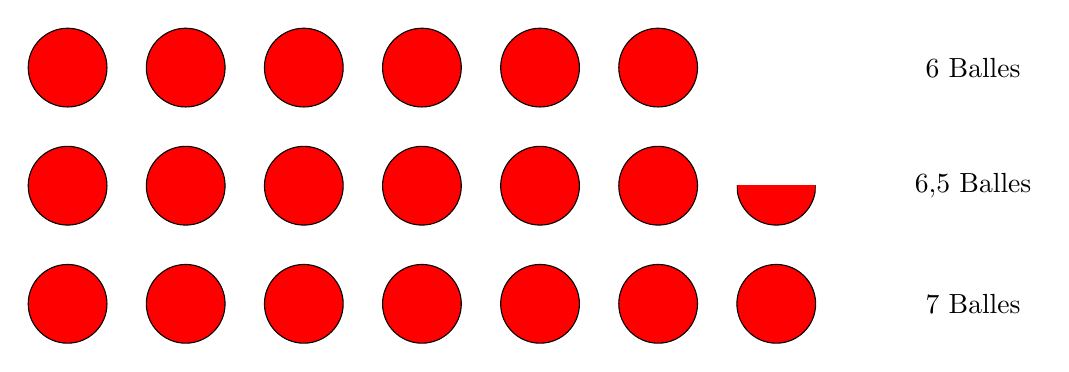
\begin{tikzpicture}
    \foreach \x in {0,1.5,3,4.5,6,7.5}
    \draw[fill=red] (\x,0) circle[radius=0.5cm];
    \draw (11.5,0) node {$6$ Balles};

    \foreach \x in {0,1.5,3,4.5,6,7.5}
    \draw[fill=red] (\x,-1.5) circle[radius=0.5cm];

    \begin{scope}
      \clip (8.5,-2.0) rectangle (9.5, -1.5);
      \draw[fill=red] (9,-1.5) circle[radius=0.5cm];
    \end{scope}
    \draw (11.5,-1.5) node {$6{,}5$ Balles};

    \foreach \x in {0,1.5,3,4.5,6,7.5,9}
    \draw[fill=red] (\x,-3.0) circle[radius=0.5cm];
    \draw (11.5,-3.0) node {$7$ Balles};
  \end{tikzpicture}

\vspace{-2cm}

\begin{tikzpicture}[overlay, remember picture]
	\draw (7.5,0) node {\includegraphics[width=3cm]{imgs/penguin7.png}};
	\draw (8.5,2.5) node[ellipse callout,draw,fill=white,font=\Large,callout absolute pointer={(8.0,0.5)},align=center] {OH!!!};
\end{tikzpicture}

% TODO: Add 2 exercises with komi and captures.
\newpage

Qui a gagné?

\cleargoban
\largegoban
\gobansize{9}
\black{e5,f3,c7,d7,e8,e6,b6,c8,c5,d2,b4,a3,a4,g5,h4,e3,d5,h3,j2,h2,f6,b9,b8,f4,e1,d3}
\white{d6,g7,c6,e7,f8,f7,d8,e9,c3,c2,b3,a2,b1,h5,h6,d4,j4,j3,j5,g6,c9,d9,e4,d1,c1,c4}
\clear{e8} % black
\clear{c6,d6} % white
\showgoban[a1,i9]

\begin{tikzpicture}[remember picture, overlay]
	\draw (6,2) node[font=\normalsize] {Prisonniers de Noir: \whitestone \whitestone};
	\draw (6,7) node[font=\normalsize] {Prisonnier de Blanc: \blackstone};
\end{tikzpicture}

\vspace{-0.5cm}
{
	\Large Blanc a \smallrectangle $-$ \smallrectangle $+$ \smallrectangle $=$ \smallrectangle points.
	
	\vspace{0.5cm}
	
	Noir a \smallrectangle $-$ \smallrectangle $=$ \smallrectangle points.
	
	\vspace{0.4cm}
	
	\rule{60pt}{2pt} gagne.
}

\begin{tikzpicture}[remember picture, overlay]
	\draw (-2.9,5.3) node[font=\small] {Territoire};
	\draw (-0.9,5.3) node[font=\small] {Prisonniers};
	\draw (1, 5.3) node[font=\small] {Komi};
	
	\draw (-2.0,3.5) node[font=\small] {Territoire};
	\draw (0,3.5) node[font=\small] {Prisonniers};
\end{tikzpicture}

\begin{tikzpicture}[overlay, remember picture]
	\draw (-5,5+3) node {\includegraphics[width=3cm]{imgs/penguin1.png}};
	\draw (-6.5,7.5+3) node[ellipse callout,draw,fill=white,font=\Large,callout absolute pointer={(-5.4,6+3)},align=center] {Prends ton temps\\pour compter!};
\end{tikzpicture}

\vspace{-2.6cm}

\noindent\rule{\textwidth}{2pt}

\vspace{-0.15cm}

Qui a gagné?

\cleargoban
\largegoban
\gobansize{9}
\black{f6,c7,c3,c4,d5,e6,f2,e3,d2,c2,f7,e8,d9,d8,c1,d6}
\white{d4,g3,g7,g6,f5,e4,e2,d3,f3,e1,f8,g8,e9,f9,d1,e5}
\clear{e3} %black
\showgoban[a1,i9]

\begin{tikzpicture}[remember picture, overlay]
	\draw (5.8,5) node[font=\normalsize] {Prisonnier de Noir:};
	\draw (6,7) node[font=\normalsize] {Prisonniers de Blanc: \blackstone};
\end{tikzpicture}

\begin{tikzpicture}[overlay, remember picture]
	\draw (5-1,5-4) node {\includegraphics[width=3cm]{imgs/penguin32.png}};
	\draw (7.5,7.5-4) node[ellipse callout,draw,fill=white,font=\Large,callout absolute pointer={(5.4,6-4.5)},align=center,inner sep=0pt] {La pierre ne peut\\ pas s'échapper.\\Cela fait un prisonnier\\pour Blanc.};
	\draw[->,ultra thick] (3.5,1.25) -- (1.1,3.0);
\end{tikzpicture}

\vspace{-1.25cm}

{\vspace{-0.475cm}
	\hspace{-5cm}{\Large Blanc a \smallrectangle $-$ \smallrectangle $+$ \smallrectangle $=$ \smallrectangle points.
		
		\vspace{0.4cm}
		
		\hspace{-5cm}Noir a \smallrectangle $-$ \smallrectangle $=$ \smallrectangle points.
		
		\vspace{0.4cm}
		
		\hspace{-5cm}\rule{60pt}{2pt} gagne.
}}
\begin{tikzpicture}[remember picture, overlay]
	\draw (-4.85,4.1) node[font=\small] {Territoire};
	\draw (-2.9,4.1) node[font=\small] {Prisonniers};
	\draw (-1.0, 4.1) node[font=\small] {Komi};
	
	\draw (-4.1,2.4) node[font=\small] {Territoire};
	\draw (-2.1,2.4) node[font=\small] {Prisonniers};
\end{tikzpicture}        
\end{center}
} % Very ugly, but this closes the \Huge


\newpage
{\huge
\begin{center}
	Jouer à Atari Go
\begin{enumerate}
	\item Joue avec un ami.
	\item L'un prend les noirs et l'autre prend les blancs.
	\item Ce sont les noirs qui commencent.
	\item Chacun pose une pierre lorsque vient son tour de jouer.
	\item Le premier qui capture a gagné.
	\item Tu peux varier les règles: capture! Au moins une pierre, capture exactement une pierre, en capturer deux, etc.
	\item Tu peux poser des pierres, ou bien dessiner. 
	\item Si tu as envie, donne des visages amusants aux pierres.

	
	
\begin{tikzpicture}[scale=0.3]
		% Second white stone
		\draw[black,fill=white] (8,10) circle[radius=0.97cm];
		
		%% Eyes
		\draw[black,fill=black] (7.6,10.4) circle[radius=0.1cm];
		\draw[black,fill=black] (8.4,10.4) circle[radius=0.1cm];
		
		%% Mouth
		
		\draw[black, ultra thick] (7.2,10) parabola[parabola height=-0.75cm] (8.8,10);
	\end{tikzpicture}
	
\begin{tikzpicture}[scale=0.3]
		% First black stone
		\draw[black,fill=black] (10,10) circle[radius=0.97cm];
		
		%% Eyes
		\draw[white,fill=white] (9.6,10.4) circle[radius=0.1cm];
		\draw[white,fill=white] (10.4,10.4) circle[radius=0.1cm];
		
		%% Mouth
		\draw[white,fill=white,ultra thick] (9.5, 9.7) -- (10.5, 9.5);
		
		%% Eyebrows
		
		\draw[white,fill=white, ultra thick] (9.9, 10.4) -- (9.4,10.7);
		\draw[white,fill=white, ultra thick] (10.1, 10.4) -- (10.6,10.7);
	\end{tikzpicture}
\end{enumerate}



\begin{tikzpicture}[overlay, remember picture]
	\draw (0,-5) node (penguin) {\includegraphics[width=3.0cm]{imgs/penguin1.png}};
	\draw (3.0,-2.5) node[ellipse callout,draw,fill=white,font=\Large,callout absolute pointer={(0.25,-4.5)},align=center,inner sep=0] {Imprime encore\\la page suivante\\pour jouer\\plus de parties!};
\end{tikzpicture}


\newpage

\vspace*{3cm}
	
	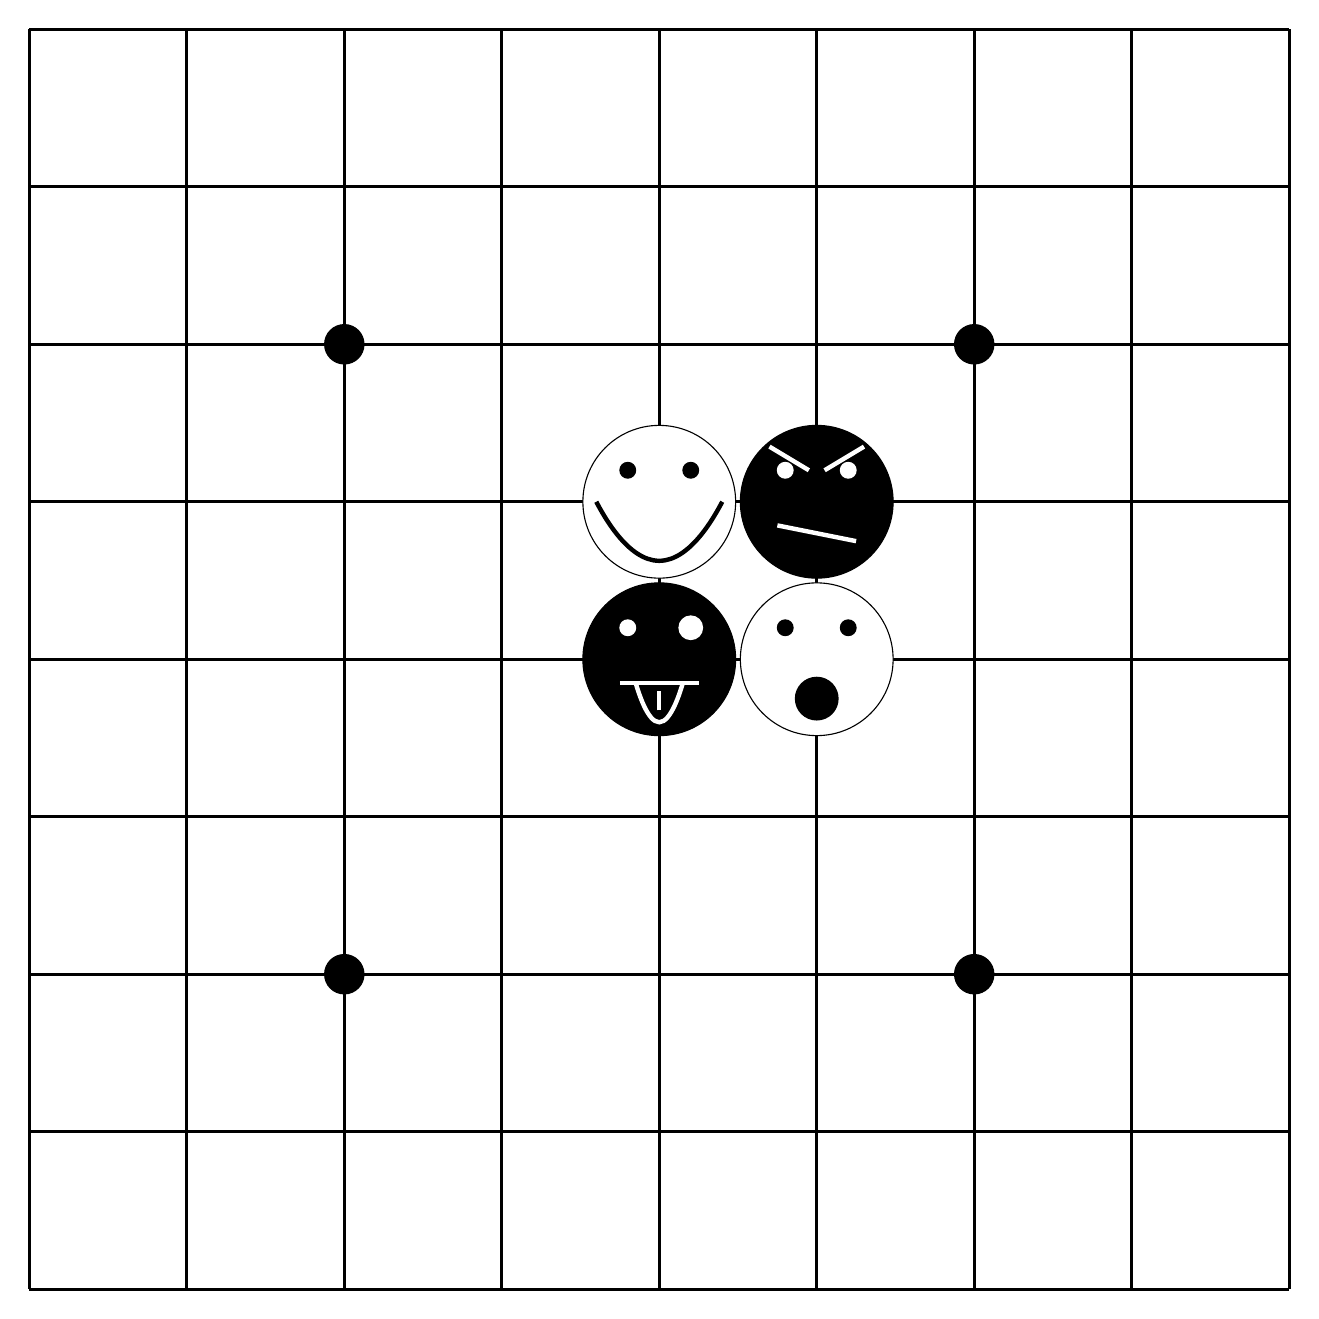
\begin{tikzpicture}
		
		\draw[very thick] grid[step=2] (16,16);
		
		\draw[black,fill=black] (4,4) circle[radius=0.25cm];
		\draw[black,fill=black] (12,4) circle[radius=0.25cm];
		\draw[black,fill=black] (4,12) circle[radius=0.25cm];
		\draw[black,fill=black] (12,12) circle[radius=0.25cm];
		\draw[black,fill=black] (8,8) circle[radius=0.25cm];
		
		% First black stone
		\draw[black,fill=black] (10,10) circle[radius=0.97cm];
		
		%% Eyes
		\draw[white,fill=white] (9.6,10.4) circle[radius=0.1cm];
		\draw[white,fill=white] (10.4,10.4) circle[radius=0.1cm];
		
		%% Mouth
		\draw[white,fill=white,ultra thick] (9.5, 9.7) -- (10.5, 9.5);
		
		%% Eyebrows
		
		\draw[white,fill=white, ultra thick] (9.9, 10.4) -- (9.4,10.7);
		\draw[white,fill=white, ultra thick] (10.1, 10.4) -- (10.6,10.7);
		
		
		% Second black stone
		\draw[black,fill=black] (8,8) circle[radius=0.97cm];
		
		%% Eyes
		\draw[white,fill=white] (7.6,8.4) circle[radius=0.1cm];
		\draw[white,fill=white] (8.4,8.4) circle[radius=0.15cm];
		
		%% Mouth
		\draw[white, fill=white,ultra thick] (7.5,7.7) -- (8.5,7.7);
		
		%% Tongue
		\draw[white, ultra thick] (7.7, 7.7) parabola[parabola height=-0.5cm] (8.3,7.7);
		\draw[white, ultra thick] (8, 7.35) -- (8, 7.6);
		
		% First white stone
		\draw[black,fill=white] (10,8) circle[radius=0.97cm];
		
		% Eyes
		\draw[black,fill=black] (9.6,8.4) circle[radius=0.1cm];
		\draw[black,fill=black] (10.4,8.4) circle[radius=0.1cm];
		
		% Mouth
		\draw[black,fill=black, ultra thick] (10,7.5) circle[radius=0.25cm];
		
		% Second white stone
		\draw[black,fill=white] (8,10) circle[radius=0.97cm];
		
		%% Eyes
		\draw[black,fill=black] (7.6,10.4) circle[radius=0.1cm];
		\draw[black,fill=black] (8.4,10.4) circle[radius=0.1cm];
		
		%% Mouth
		
		\draw[black, ultra thick] (7.2,10) parabola[parabola height=-0.75cm] (8.8,10);
		
	\end{tikzpicture}
\end{center}

} % Very ugly, but this closes the \Huge

\newpage


\section*{Crédits}
La plupart des images viennent de Open Clipart (\url{https://openclipart.org}) et sont dans le domaine public:

\vspace{0.25cm}

\noindent\hspace{-0.5cm}\begin{minipage}{10cm}
\begin{itemize}
\item Main dessinant: j4p4n (\url{https://openclipart.org/detail/321385/doodling-hand}).
\item Manchot confus: zafx (\url{https://openclipart.org/detail/169173/basetuxg2v12}).
\item Autres manchots: Moini (e.g., \url{https://openclipart.org/detail/174879/wild-penguin}).
\end{itemize}
\end{minipage}

\vspace{0.25cm}

L'image du goban en couverte est une capture d'\'{e}cran de l'application ``Sabaki'' application \url{https://github.com/SabakiHQ/Sabaki}. La partie montr\'{e}e date de 2021, entre Lukáš Podpěra et Stanisław Frejlak lors de la finale de la 6th European Pro Qualification. 

Ce livre fut fait en \LaTeX, avec notamment les paquets \emph{Igo} pour les diagrammes et \emph{TikZ} pour la mise en page.

Je remercie Ai Guan, Björn Eurenius et Florian Pein pour avoir relu la version de travail.

\section*{Distribution}

Ce livre est disponible sous la licence Creative Commons BY-NC\_SA 4.0. Vous pouvez le distribuer librement.

Il est disponible depuis mon site web: \url{www.leandromarcolino.com.br}. Le code source est disponible sur GitHub (\url{https://github.com/sorianom/kids-go-books}).

Si vous aimez ce livre et que vous souhaitez me l'exprimer, vous pouvez m'offrir un caf\'{e} via \url{https://buymeacoffee.com/leandromarcolino}.

\bigskip

\begin{center}
  \href{https://buymeacoffee.com/leandromarcolino}{\includegraphics[width=5.0cm]{imgs/bmc-button.png}}\\
  \url{https://buymeacoffee.com/leandromarcolino}
\end{center}

\newpage
\thispagestyle{empty}
\
\newpage

\begin{center}
\begin{tikzpicture}[overlay, remember picture]

\draw (0,-12) node[opacity=1.0] {\includegraphics[width=1.85\columnwidth]{imgs/goBoard.png}};
  
%\draw (0,-12) node  {\includegraphics[width=1.5\columnwidth]{imgs/penguins.png}};

\end{tikzpicture}
\thispagestyle{empty}
%% \vspace{-2.5cm}

%% {{\fontsize{100}{110}\selectfont \contour{red}{Mon premier livre de}\\
%%   \contour{red}{Go Exercises}}}
  
%% \vspace{20cm}
%%        {{\fontsize{40}{50}\selectfont \contour{white}{By: Daddy}}}
%%        \thispagestyle{empty}
%% \end{center}
\end{center}
\end{document}
